\chapter{DNA Models}
\label{chap:dna}


\section{3SPN.2C}
\label{sec:dna_3spn2c}

The series of the 3SPN.x DNA models have been developed by de Pablo's group.
The 3SPN.2C model is the one for modeling sequence-dependent curvature of
double-stranded DNA (dsDNA).  Particularly, the model has been well-tuned to
reproduce both mechanical and geometrical properties, such as persistent length
and major/minor groove widths.

\subsection{Topology}
\label{subsec:dna_3spn2c_top}

In this model, each nucleotide is represented by three CG particles, P
(phosphate), S (sugar), and B (base), as shown in
Figure~\ref{fig:dna_3spn2c_top}.  B has four types: A (adenine), C (cytosine), G
(guanine), and T (thymine).  The CG particles are put at the center-of-mass of
each chemical moiety.

\begin{figure}[ht]
  \centering
  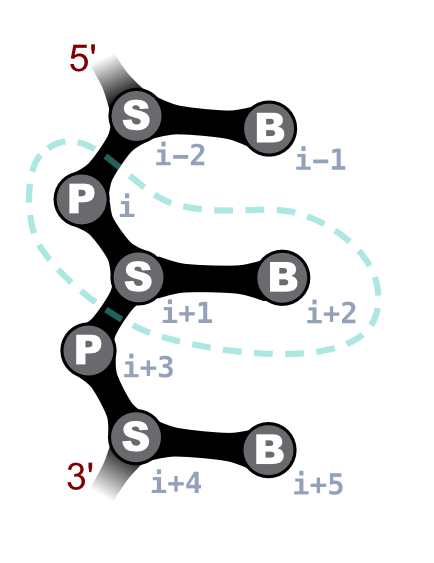
\includegraphics[width=0.3\textwidth]{figures/DNA_3spn2c_top.png}
  \caption{Topology of the 3SPN.2C DNA model: each nucleotide is represented by
    3 sites corresponding to phosphate (P), deoxyribose sugar (S), and
    nitrogenous base (B).  A typical nucleotide ``residue'' is enclosed by the
    dashed line.}
  \label{fig:dna_3spn2c_top}
\end{figure}


\begin{table}[ht]
  \centering
  \begin{tabular}{lc}
    \toprule
    Particle Type    & Mass (amu) \\
    \midrule
    P  &  94.97 \\
    S  &  83.11 \\
    A  &  134.1 \\
    C  &  110.1 \\
    G  &  150.1 \\
    T  &  125.1 \\
    \bottomrule
  \end{tabular}
  \caption{Mass of the 3SPN.2C DNA particles.}
  \label{tab:dna_3spn2c_top_mass}
\end{table}